\documentclass[11pt,twoside]{eitExjobb}
%%\documentclass[11pt,twoside,final]{eitExjobb}  % Use final for the final version that will be printed
%%%%%%%%%%%%%%%%%%%%%%%%%%%%%%%%%%%%%%%%%%%%%%%%%%%%
%% Other fonts (Palatino as rm font, helvetica as sf font and courier as tt font. All fonts are normally installed with a standard LaTeX distribution.)
% \usepackage{mathpazo} % Also in math mode
% \usepackage[scaled=.95]{helvet}
% \usepackage{courier}
%%%%%%%%%%%%%%%%%%%%%%%%%%%%%
% ÅÄÖ
\usepackage[utf8]{inputenc}  % Input encoding (this file): 8 bit unicode. Default by most text editors
\usepackage[T1]{fontenc}     % Output encoding (pdf file)
%%%%%%%%%%%%%%%%%%%%%%%%%%%%%
%% Packages used in the example
\usepackage{graphicx}   % Included graphics and some resizable boxes
\usepackage{url}        % nice urls with line breaks
\usepackage{lipsum}     % nonsense text blocks
\usepackage{listings}
\usepackage{float}
\usepackage{enumitem}
\usepackage{amsmath} 
%%%%%%%%%%%%%%%%%%%%%%%%%%%%%%
%%%%%%%%%%%%%%%%%%%%%%%%%%%%%%
%%%%%%%%%%%%%%%%%%%%%%%%%%%%%%
\lstset{
    frameround=fttt,
    numbers=left,
    breaklines=true,
    captionpos=b,
    keywordstyle=\color{blue}\bfseries, 
    basicstyle=\ttfamily\color{black},
    numberstyle=\color{black}
}
\lstMakeShortInline[columns=fixed]|

\begin{document}

	\Title{Evaluating Analytic Wi-Fi Performance Models Based on End-User Data}
	\Author{Axel Smeets\\\texttt{dat12asm@student.lu.se}}
	\Supervisor{Björn Landfeld}
	\Examiner{Christian Nyberg}

	\MakeTitlePage
	\frontmatter

	\chapter*{Acknowledgements}
	hello

	%!TEX root = report.tex

\chapter*{Abstract}

The performance characteristics of Wi-Fi networks have traditionally been
studied and analysed using analytical models and simulations. Due to the
complexity of wireless communication the existing analytical Wi-Fi network
models rely on certain network constraints and simplifications in order to be
mathematically tractable.

We set out to evaluate the practicality of using Wi-Fi performance models to 
estimate network performance by collecting the necessary parameters directly
from an access point. By extension, we must also collect network metrics,
such as packet payload size and number of nodes, for comparison with the model. We 
explore different venues to collect these parameters and metrics to find out
if it is practical to apply the models in Wi-Fi networks. 

After performing three attempts, we conclude that this is difficult due to
several aspects in the Linux kernel, such as batching optimization patterns,
proprietary kernel modules and firmware blobs.


	%!TEX root = base.tex

\chapter*{Popular Science Summary}

% Trådlös kommunikation har växt explosionsartat de senaste årtionden och
% konsumenters krav och förväntningar på bandbredd ökar allt mer. I många hem
% finns trådlösa accesspunkter med stöd för Wi-Fi. De kommer i många skepnader
% - inbakade i en router, som komplement vid sidan av eller i form av s.k.
% "Repeaters".

% Majoriteten av accesspunkter och apparater implementerar Wi-Fi b/g/n vilka kommunicerar via
% radio över frekvensband vid 2.4 GHz. Många modernare accesspunkter lägger även
% till stöd för Wi-Fi ac med frekvensband vid 5 GHz.

% Radiovågors räckvidd är direkt beroende på våglängden och skillnaden i räckvidd
% mellan 2.4 GHz och 5 GHz vara mycket stor. Detta medför att accesspunkter i
% ett hus kan nå in i grannhuset eller lägenheterna runt omkring, och därmed störa
% den trådlösa kommunikationen där, och vice versa.

% För att minimera effekten av denna interferens utnyttjar inte varje accesspunkt
% hela frekvensbandet som standarden tillåter. Istället ska accesspunkterna
% konfigureras så att närliggande accesspunkter inte använder samma del av
% frekvensbandet.

% Det inte finns någon central myndighet, samordning bland tjänsteleverantörer
% eller grannar emellan som genomför denna konfiguration och det är alltså upp
% till den enskilde.

% En stor del av hur en användare upplever nätverket kan därför direkt påverkas av
% hur deras accesspunkt är konfigurerad. Är det många grannar som pratar på samma
% kanaler leder detta till nedsatt prestanda, vilket kan visa sig på många olika
% sätt.

% När kunden inte är nöjd ringer de tjänsteleverantörens support och försöker få
% hjälp. Detta kostar företagen miljonbelopp varje år och oftast måste en tekniker
% skickas ut för att försöka lösa problemet, som egentligen inte ligger på
% leverantörens del av nätet.

% Denna studie har använd data från Telenor med existerande modeller av Wi-Fi-nät
% för att undersöka deras uppförande och se om de överhuvudtaget går att använda.

% Studien har även tagit ett steg till och undersökt om och hur dessa modeller kan
% användas för att estimera Wi-Fi-nätets prestanda vid vissa typer av
% förändringar, t.ex. antalet grannstationer.


	\tableofcontents
	\listoffigures
	\listoftables
	\cleardoublepage

	\mainmatter

		\chapter{Introduction}

In 2014 a report on Wi-Fi adoption found that 25\% of households, all over the
world, had Wi-Fi networks set up. In households with fixed-line broadband
access, 65\% had set up a Wi-Fi network\cite{smith}. The report also states that
the number of Wi-Fi-enabled devices is projected to increase.

Naturally, consumers today have higher expectations regarding network throughput
and latency than the IEEE 802.11 standard was designed for back in 1997. In
recent years, the Wi-Fi label has become hugely popular and the standard been
catching up ever since it was introduced beyond the corporate sector, for which
it was originally intended, with almost annual extensions.

One limitation all wireless networking technologies have to consider is radio
interference. Some protocols implement ALOHA-style protocols with no
coordination between devices, relying on collision detection techniques and
subsequent retransmission. IEEE 802.11 implements a \emph{distributed
contribution function} (DCF) which is resposible for controlling access to the
medium.

Even though newer routers today are able to automatically (re)configure
themselves based on analysis of neighbouring networks, they are not guaranteed
to be optimal since they have a local view of the network. Older routers rely on
manual configuration. This configuration is not strictly an issue with the
standard, but rather with how the routers are being deployed. One can think of
the deployment process as being decentralised—each household purchases and
configures their own router.

With existing IEEE 802.11 models it is possible to predict configuration
effects. However, few, if not none, implementations conform to the theoretical
models. This work aims to evaluate IEEE 802.11 models with end-user data and
analyse if, and how, these models may be applicable.

% Centralised configuration is still not on the map for the foreseeable future. Expert systems are already in-place. The task becomes on how to improve existing systems---can we come up with a system which guarantees that a recommended change results in an improvement? This would require extensive simulation of the network and the ability to predict the effect of a change in a configuration parameter.




This master thesis aims to be a step in this direction: evaluate existing Wi-Fi models to see if they are useful in real-world settings.
% em —


% Recommend configuration based on both detailed and wide view of network performance.

% To recommend a change it must lead to improvement in some aspect.

% How to be sure of this? Model the network and simulate what happens when the change is made.

% This requires competent Wi-Fi models.

% Must have clear definition of a competent Wi-Fi model is.

% Wi-Fi models with good performance in simulated tests need not be as good in the real world.

% So we have to test this, and we need the data to do it.

% Telenor now has a good platform for us to get the data.

% But can we trust it? Perhaps the logging is inaccurate?

% So we need to analyse the quality of the data.

%  - is it accurate?
%  - is it precise?

% Experiments will be conducted and results will impact model testing and evaluation.


		\chapter{Background}

This chapter provides an overview of the related topics for this master thesis.

\section{TG799-vac}

The OpenWrt-based router examined in this thesis, see Figure \ref{fig:tg799}, is commonly known as TG799, manufactured by Technicolor with Broadcom and Quantenna modems. A custom firmware was used to gain root access over SSH.

\begin{figure}
\center
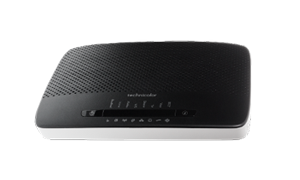
\includegraphics[width=0.5\textwidth]{images/tg799.png}
\caption{The TG799 router from Technicolor}
\label{fig:tg799}
\end{figure}

\section{IEEE 802.11}

The ubiquitous set of LAN standards for wireless communication. Specify MAC and PHY protocols.

Basic protocol description, relevant for this master thesis.

How later standards IEEE 802.11b g n ac change.

\section{ubus - the OpenWrt micro bus architecture}

A client program which acts as an interface to the bus daemon, \texttt{ubusd}. Input and output format is JSON.

The router registers a namespace called \texttt{wireless} and this is what we call to find the meaning of life.

\section{Deutche telekom supra}

Björns oklara vapen.

\section{Rhode \& Schwarz FWLZ-XYZ}

(not broken) network analyser;

\section{Wi-Spy Channalyzer}

the wi-spy, top secret agent auf d00m.

\section{Wireshark}

Wireshark is a well-known program for capturing and inspecting network data.


		%!TEX root = base.tex

\chapter{Previous Work}

Modelling of Wi-Fi performance has been an active field of research and this
chapter provides an introduction to the modeling approach described by Bianchi
\cite{bianchi} and subsequent efforts to improve it made by others. In
particular, the studied model presented by Ekici \& Felemban \cite{felemban}
will be discussed.

As mentioned previously, the IEEE 802.11 family specifies the PHY and MAC
layers of WLANs. Analysing the performance impact of these protocols, and 
their numerous parameters, is key to improving network performance. There are
two possible paradigms available: measuring/sampling or constructing an
analytic model of the system/property. Measuring can be done directly on both
physical hardware and software simulations whereas analytical models provide
performance figures as solutions of equations.

The complete behavior of the IEEE 802.11 standards have yet to be captured by
any single analytic model, and researchers instead take the standard
scientific approach of solving a constrained variant of the problem, which in
turn requires rigorous validation of the solution. A model may perform well in
certain conditions and pathologically in others. These behavioural
pecularities arrise from simplification of system behaviour and properties. In
a given model, simplifications can also be inherent in the original
construction mechanism—the way the model itself was constructed—which forces
the model itself to undergo a sort of ironic self-analysis and validation.
Model authors typically present a validation effort to prove their model's
credibility, which further requires scrutiny of the validation itself,
possibly in absurdum...

In short, model authors try to describe a complex system by modelling key
components in a constrained setting, and validate their model using other
models which have been more thoroughly reviewed. 

Given this context, we first present the original Markov-Chain model from
\cite{bianchi} and describe how it models IEEE 802.11 properties using the
DCF, some significant and intentional simplifications made and a narrow
selection of subsequent contributions made by others $refs$. % TODO: ADD REFS

Finally, the evaluated model \cite{felemban} is described as well as the
differences to both the original model \cite{bianchi} and some intrinsic model
properties useful in forthcoming chapters.

\section{The Bianchi Model}

In \cite{bianchi}, Bianchi presented a novel approach to modeling IEEE 802.11
performance by creating a Markov chain model of the \emph{Distributed
Coordination Function} (DCF). Bianchi defines three important properties:
transmission probability, normalised throughput and channel access delay. This
section provides a summary of the original model and definitions useful in
later chapters.

Before going into detail about the Bianchi model, we start from the beginning.

The underlying assumption of a MAC-layer-based model of IEEE 802.11 is that,
in a setting with more than 2 STAs, the MAC protocol should be the system
bottleneck. By extension, it is reasonable to model the performance of the
network based on the DCF. 

In \cite{bianchi}, Bianchi starts by limiting the proposed model analysis to
fully-connected, single-hop networks in ``saturation''. The saturation
condition requires that all STAs, at any point in time, always want to
transmit. This allows Bianchi to omit send queue distributions and simplify
collision probabilities, which will become important. Additionally, Bianchi
assumes that there is a fixed number of $N$ equivalent, contending STAs.

The back-off counter for a given STA at time $t$ is represented by the
stochastic process $b(t)$. Since the back-off counter at any given time $t$ is
dependent on the transmission history it follows that $b(t)$ is non-Markovian.
To solve this problem Bianchi assumes that each transmission attempt collides
with a constant and independent probability $p$.

In addition to the back-off counter process, $b(t)$, Bianchi also introduces a
stochastic process $s(t)$ representing the current back-off stage for a given
STA at time $t$. Recall from Equation \ref{eq:mlog} that $m$ is the number of
back-off stages, from which the states of $s(t)$ can be obtained as $(0,
\dots, m)$.

After breaking the historical dependency of the back-off process, Bianchi can
model the time-discrete bidimensional process $\{s(t), b(t)\}$ as the Markov
chain seen in Figure \ref{fig:tnmc}. As seen in the figure, the model ignores
several important behaviors of the DCF, in particular retransmission limit and
backoff counter freezing due to channel state.

\begin{enumerate}

	\item \textbf{Retransmission Limit} - the model does not drop the packet
after failing \texttt{ShortRetryLimit} retransmissions, instead it continues
until the packet has been successfuly acknowledged.

	\item \textbf{Back-off Counter Freezing} - in each back-off state, the
probability of decrementing the back-off counter—equivalent to sensing the
channel idle—is always 1.

\end{enumerate}

Bianchi assumes that the conditional collision probability $p$ is constant and
independent of the back-off stage. This implies that $p$, the probability of
an STA encountering collision during transmission, is equivalent to the
probability that any of the other $N-1$ STAs also attempted to transmit, with
transmission probability $\tau$

\begin{equation} \label{eq:pbi}
	p = 1 - (1 - \tau)^{N-1}
\end{equation}

By modelling the back-off counter itself, combined with the saturation
condition and omission of retransmission limit, Bianchi solves the
transmission probability $\tau$ by essentially finding the steady state
probability of the back-off counter being zero, and obtains

\begin{equation} \label{eq:xbi}
	\tau = \frac{2(1-2p)}{(1-2p)(\mathit{CW_{min}}+1)+p\mathit{CW_{min}}(1-(2p)^m)}
\end{equation}

However, since $\tau$ is derived from the back-off counter, and the back-off
counter depends on the conditional collision probability $p$, it follows that
$\tau$ and $p$ are recursively defined. Bianchi constructs a nonlinear system
with equations for $\tau$ and $p$ and solves it numerically.

With probabilities for $\tau$ and $p$, Bianchi continues to his core
contribution—the normalised throughput. Denoted $S$, it is defined as ``the
fraction of time the channel is used to transmit payload bits''. 

\begin{equation} \label{eq:ssbi}
	S = \frac{E[\mathit{payload~information~transmitted~in~a~slot~time}]}{E[\mathit{length~of~slot~time}]}
\end{equation}

With $E[P]$ denoting mean payload size, probabilities for transmission
$P_{tr}$ and transmission success $P_S$, the numerator in \ref{eq:ssbi}
becomes $P_S P_{tr} E[P]$. In a similar fashion, the denominator in
\ref{eq:ssbi} can be expressed as the sum of empty time slots, busy time slots
and times slots with collisions. Let $\sigma$ be the duration of an empty
slot, $T_{S}$ the average time the channel is sensed busy in case of
successful transmission, and $T_{C}$ the average time the channel is sensed
busy in case of collision for the non-colliding STAs. Now, Bianchi presents an
equation for the normalized througput $S$

\begin{equation} \label{eq:sbi}
	S = \frac{P_S P_{tr} E[P]}{(1-P_{tr})\sigma + P_{tr} P_S T_S + P_{tr} (1-P_S) T_C}
\end{equation}

Note that $S$ is expressed independent from the ``access modes'' found in
Figure \ref{fig:timings}, which details the communication flow of a single,
successful packet transmission and acknowledgement. Let $H = T_{\mathit{PHY}}
+ T_{\mathit{MAC}}$ and assume propagation delay $\delta$. The differences
between the ``access modes'' can thus captured by the variables $T_{S}$ and
$T_{C}$

\begin{align}  \label{eq:tbi}
	\mathit{basic} & \left\{
		\begin{aligned}
	        T^{bas}_{S} & = H + E[P] + \mathit{SIFS} + \delta + \mathit{ACK} + \mathit{DIFS} + \delta  \\
	        T^{bas}_{C} & = H + E[P] + \mathit{DIFS} + \delta
	    \end{aligned}
	\right. \\
	\mathit{RTS/CTS} & \left\{
	    \begin{aligned}
	        T^{rts}_{S} = & ~ \mathit{RTS} + \mathit{SIFS} + \delta + \mathit{CTS} + \mathit{SIFS} + \delta \\ & + H + E[P] + \mathit{SIFS} + \delta + \mathit{ACK} + \mathit{DIFS} + \delta  \\
	        T^{rts}_{C} = & ~ \mathit{RTS} + \mathit{DIFS} + \delta
	    \end{aligned}
	\right.
\end{align}


From these equations Bianchi concludes that for any network of size $N$ there
exists a troughput-optimal transmission probability $\tau$, achievable by
tuning the congestion window sizes and $\mathit{CW_{min}}$ and $\mathit{CW_{max}}$.

To make the model tractable Bianchi simplifies many behaviours, of which two
have received considerable efforts to implement. Some notable publications 
are Wu \cite{1019305} and Chatzimisios \cite{1258379}, who proposed improved
models that included the retransmission limit, followed by Zhang
\cite{article} and Xiao \cite{1512111}, who proposed models that include
back-off counter freezing.

\begin{figure}
\center
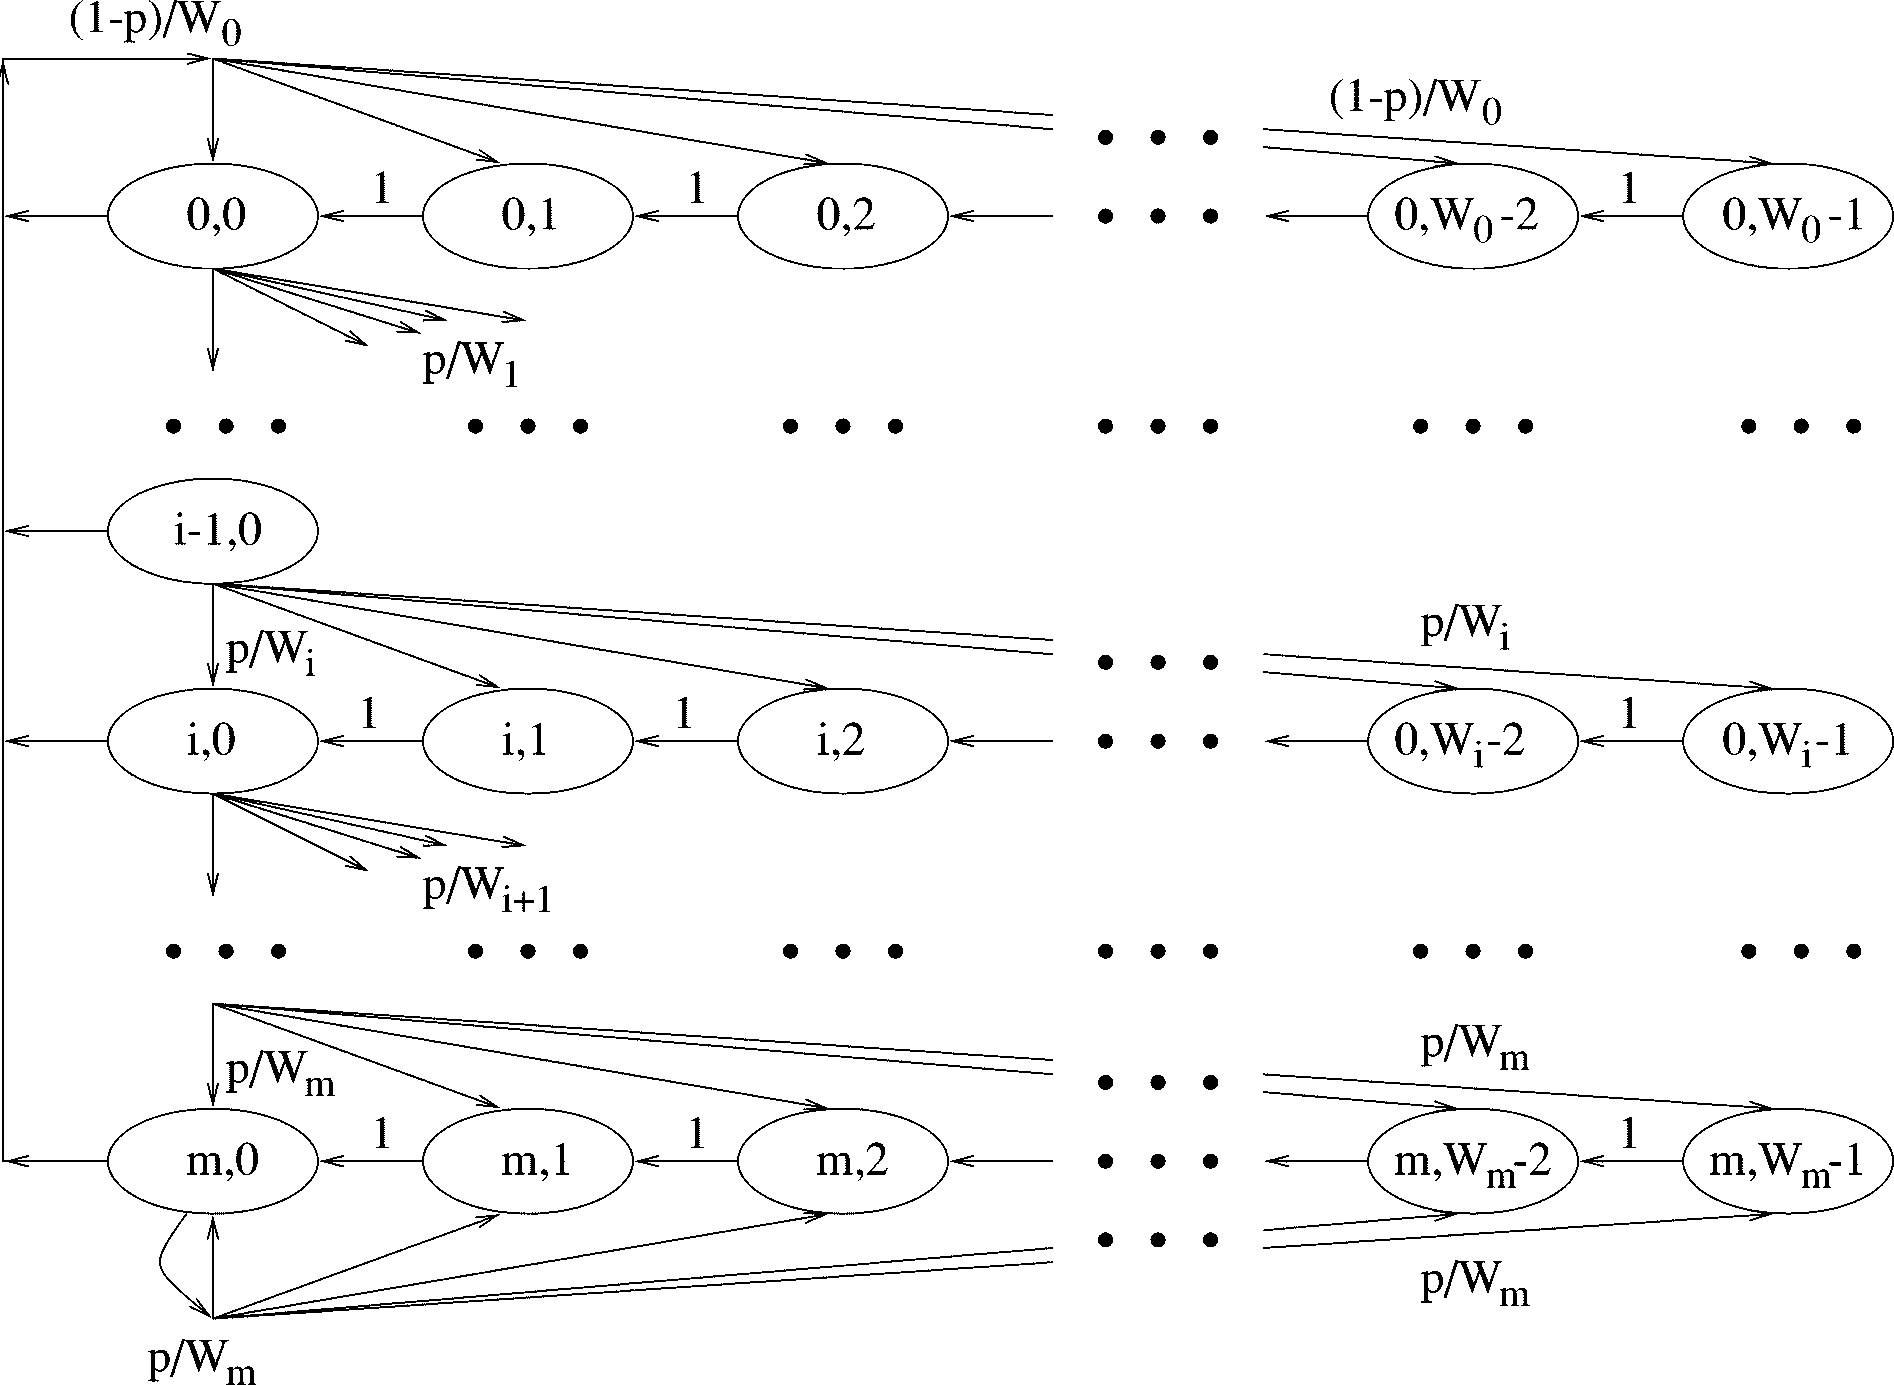
\includegraphics[width=0.9\textwidth]{images/bianchi-model.png}
\caption{Bianchi's \emph{Tagged-Node Markov Chain} model of the IEEE 802.11 DCF where $p$ is the collision probability, $W_i$ the contention window size at attempt $i$ ($0 \leq i \leq m$) and $m$ from Equation \ref{eq:mlog}.}
\label{fig:btnmc}
\end{figure}

\section{The Felemban-Ekici Model}

A decade later, in 2011 specifically, Felemban \& Ekici published an extended
version of Bianchi's model, where they significantly improved the model's
accuracy by introducing a more accurate behaviour of the entry into backoff
and the backoff countdown procedures \cite{felemban}.

An overview of the TNMC model from \cite{felemban} is presented in Figure
\ref{fig:tnmc}. Some differences compared to Bianchi's TNMC are inclusion of
retransmission limit (in state $\{0,L\}$, collision results in packet drop)
and counter freezing $P_f$ (probability of state a $\{i,j\}$ transitioning to itself).

The inclusion of retransmission limits results in a different expression of
$\tau$ compared to Equation \ref{eq:xbi}. Recall from Equation \ref{eq:cwj}
that $W_j$ is the size of the contention window at back-off stage $j$ and that
$L$ is the short retry limit from \cite{654749}. Felemban \& Ekici solves
$\tau$ similarly to \cite{bianchi} by finding the probability of the back-off
counter reaching 0 in all back-off stages, expressed as

\begin{equation} \label{eq:xfe}
	\tau = \frac{1-P^{L+1}}{
		(\Sigma^L_{j=0}
			[1 + \frac{1}{1-P_f}
				\Sigma^{W_j-1}_{k=1} \frac{W_j-k}{W_j}
			]
		)(1-P)}
\end{equation}

where $P$ is the conditional collision probability (equivalent to $p$) from
Equation \ref{eq:pbi}.

\begin{align}  \label{eq:tfe}
	\mathit{basic} & \left\{
	        T^{bas}_{C} = T^{bas}_{S} = \mathit{DIFS} + T_h + T_p + \mathit{SIFS} + \mathit{ACK}
	\right. \\
	\mathit{RTS/CTS} & \left\{
	    \begin{aligned}
	        T^{rts}_{S} = & ~ \mathit{DIFS} + T_\mathit{RTS} + \mathit{SIFS} + T_\mathit{CTS} \\ & + \mathit{SIFS} + T_h + T_p + \mathit{SIFS} + \mathit{ACK}  \\
	        T^{rts}_{C} = & ~ \mathit{DIFS} + T_\mathit{RTS} + \mathit{SIFS} + T_\mathit{CTS}
	    \end{aligned}
	\right.
\end{align}

As shown in Figure \ref{fig:dcfgraph}, the DCF back-off process algorithm
specifies that a node only decrements the back-off counter if the channel was
sensed idle. In \cite{felemban}, the authors obtained an accurate countdown
probability ($P_d$) by introducing an additional markov chain to model the
channel-sensing process and estimating the probability of \emph{not} counting
down, i.e. probability of counter freeze ($P_f$). This chain is called
Channel-Sense Markov Chain (CSMC). The counter freeze probability, $P_f$, is
computed by finding the steady state probabilities of the CSMC by fixed point
iteration.

The addition of CSMC and $P_f$ increased the model's accuracy significantly
compared to other models in various test conditions. In particular, the
introduction of $P_f$ increased accuracy of the model when extended to
\emph{unsaturated} networks.

While the model proposed by Ekici-Felemban models the DCF more closely and
accurately, several assumptions and omissions, in addition to constraints
inherited from the markov chain approximation, makes the model a very
interesting candidate for real-world testing. 

\begin{figure}
\center
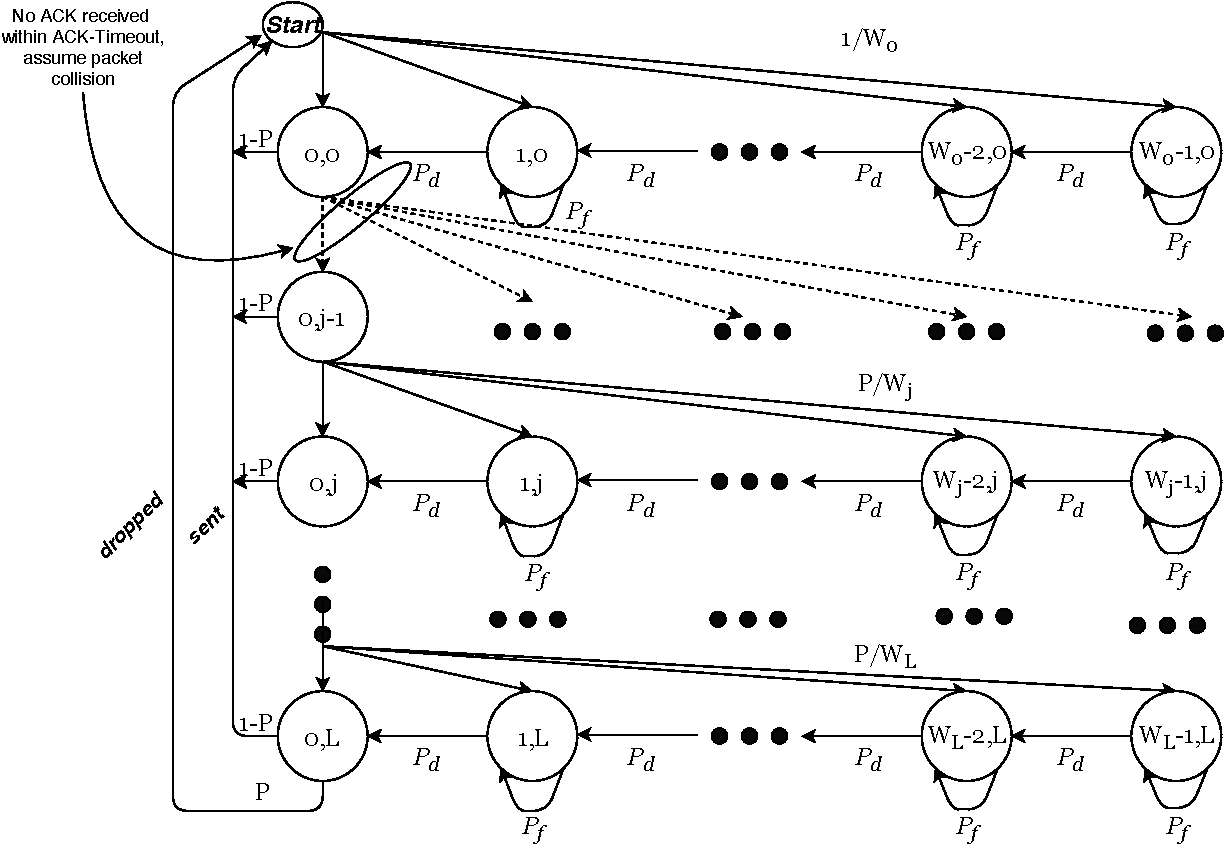
\includegraphics[width=1\textwidth]{images/tnmc-dcf.pdf}
\caption{Ekici-Felemban's Tagged-Node Markov Chain (TNMC) model of the IEEE 802.11 DCF. $P$ is packet collision probability, $P_d$ is probability to decrease backoff counter, $P_f = 1 - P_d$, $W_j$ is contention window size at attempt $j$ and $L$ is the Short Retry Limit}
\label{fig:tnmc}
\end{figure}

\subsection{The Unsaturated Model}

Recall that the original Bianchi model assumed that the network was in
\emph{saturation} conditions, i.e. all STAs always have something in their
send buffer. After presenting the improved model in \cite{felemban}, 
extended to work in \emph{unsaturated} networks.

		\chapter{Methodology}

This section describes the methodology used to analyse the models.

\section{Model Selection}

\begin{verbatim}
  +-> model selection --> list of parameters --+
  |                                            |
  +-- parameter analysis <-- data collection <-+
\end{verbatim}
 
\section{Data Collection}

The evaluated model is Felemban-Ekici.

\section{Model Parameters}
The first step was to analyse the theoretical models.

To run the Felemban-Ekici model the following properties are required:

\begin{itemize}
	\item \emph{N}, the number of network nodes
	\item $CW_{min}$ and $CW_{max}$, contention window min and max size
	\item \emph{E[D]}, the mean payload size
	\item channel bit rate
	\item $L$, the \texttt{ShortRetryLimit}
\end{itemize}

The Felemban-Ekici model provides metrics such as normalized throughput, channel access delay and probability of packet collision.

\section{Tool}

On the router side three programs, which provide access to network interface data, were tested and evaluated:

\begin{enumerate}
	\item ubus - openwrt interface
	\item qcsapi - quantenna interface
	\item wl - driver interface
\end{enumerate}

In the end, ubus was chosen as it was found to be more consistent than the qcsapi.

\section{Parameter Extraction}

In order to evaluate the models we needed these parameters:

\begin{itemize}
\item rssi
\item nodes
\item logical tx/rx rates
\item physical tx/rx rates
\end{itemize}

\section{Parameter Analysis}

We must analyse the validity of the reported parameters.

Do this with experimentation in the radio lab.

We want to analyse the reported values for RSSI, SNR, broken \& valid IEEE 802.11 frames.

Using quantenna and wl API:s to query:
\begin{itemize}
    \item \texttt{wl assoclist} $\rightarrow$ \texttt{wl rssi}
    \item \texttt{ubus call wireless.radio.monitor get}
    \item \texttt{qcsapi get\_rssi\_per\_association "wifi0"}
\end{itemize}


		In Figure~\ref{fig:testfig} a typical test mage is shown.
\begin{figure}[htbp]
  \centering
  \includegraphics[width=0.4\linewidth]{example-image}
  \caption{Example image.}
  \label{fig:testfig}
\end{figure}

\section{New new section}
\lipsum[1-2]
\begin{table}[htbp]
  \centering
  \begin{tabular}{lll}
    Group & Test 1 & Test 2\\\hline
    A & 253 &54\\
    B & 636 & 33
  \end{tabular}
  \caption{A nice table.}
  \label{tab:tabletest}
\end{table}

\lipsum[3]
\begin{figure}[htbp]
  \begin{minipage}[t]{0.5\linewidth}
    \centering
    \includegraphics[width=0.8\linewidth]{example-image-a}
    \caption{Image A}
    \label{fig:imageA}
  \end{minipage}%
  \begin{minipage}[t]{0.5\linewidth}
    \centering
    \includegraphics[width=0.8\linewidth]{example-image-b}
    \caption{Image B. It can also be a long caption even if the space is narrow.}
    \label{fig:imageB}
  \end{minipage}
\end{figure}

Figure~\ref{fig:imageA} is displayed next to Figure~\ref{fig:imageB}. Notice that \verb|\linewidth| is the line width inside the \verb|minipage|.

\lipsum[4]


		%!TEX root = report.tex

\chapter{Discussion and Future Work}

In this chapter we first discuss the experiments and their results. Then we
proceed to discuss the model based on experiments. Finally, we present some
ideas on interesting research opportunities and our closing thoughts.

\section{Discussion of results}

In this section we will comment on the results obtained, primarily from our
experiments. More importantly, we will also expand upon the discussion
presented for each experiment in the Chapter 4 where we explained our
experimental approach.

\subsection{Experiment 1: Wireshark}

As revealed in Figure \ref{fig:wstiming} (actual timing model), the design of
this experiment has a critical flaw which is not apparent without deeper
insight into the network stack. As explained earlier, the ``packet tap''
feature from which Wireshark obtains packets is triggered when the packet
exits the kernel queueing system (qdisc) and handed over to the driver for
transmission, rather than once the driver receives a transmission event from
the hardware. This completely invalidates the fundamental design model and
thus the experiment as such.

Further exploration showed that the experiment design could work if packets
could be timestamped in hardware and somehow captured after transmission.
There \emph{is} support for this in Linux, and Wireshark, but unfortunately
relies on features not available in our hardware.

The presented results are mostly included for completeness and should not be
regarded as anything useful, except for measuring system call to pcap
latencies.

\subsection{Experiment 2: Queueing the Network System}

As described in Section \ref{sec:experiment2}, there are some issues with the
definition of $W_\text{NIC}$ from Equation \ref{eq:wnic} due to a deferred
memory release mechanism in the kernel. Specifically, the definition of the
NIC queuing system from Figure \ref{fig:exp2_overview} includes a note
``kernel scheduler frees handled pkts''.

In order to increase throughput (at the expense of latency), Linux will free
up handled packets in batches. This part greatly impacts the \texttt{sndbuf}
which is used in Equation \ref{eq:sndbuf}, implying that sent or dropped
packets -- but not yet freed -- will still count as enqueued in the NIC. In
short, the modeled $L_\text{NIC}$ includes packets in driver/firmware, in
hardware and, crucially, in the kernel's to-free list.

By increasing the \texttt{sndbuf} we could observe a corresponding increase in
$L_\text{NIC}$ (and $W_\text{NIC}$) in our experiments. However, this fact
does not imply that there are not any more packets in the NIC. Recall that the
NIC queueing system actually consists of a driver/firmware queue and a
hardware queue. The hardware queue on most consumer chips is \emph{probably}
either fixed and very limited in size, or non-existant (RAM \emph{is}
expensive).

After additional analysis of the source code of Intel's open source Wi-Fi
driver, the driver/firmware queue length was determined to be 256 packets
large. By assuming a full \texttt{sndbuf} (i.e. $K$ packets in the network
system) and a full NIC, we can model $K$ as $K = L_\text{qdisc} + 256 +
\text{hardware} + \text{to-be-free}$ where \texttt{hardware} and
\texttt{to-be-freed} are unknowns.

One can argue that for the hardware queue to have any impact on the other
queues, it would have to be of similar size. Otherwise, it should be safe to
assume an interrupt-based solution: a driver manages known packets and
hardware signals which have been sent using (soft) interrupt requests (IRQ),
i.e. no dedicated hardware buffer. Thus the total queue size of the NIC is
determined by the driver, in our case $256$ packets, simplifying $K =
L_\text{qdisc} + 256 + \texttt{to-be-freed}$. This exposes the core issue with
the original queue model: there is no separation between ``in queue, waiting
to be served'' and ``served, waiting to be freed''.

In the program which logged $L_\text{qdisc}$, we could observe how many
packets were fed into the driver ``at once''. Our tests show that multiple,
10+, packets being handed over to the driver between timestamps $<10 \mu s$.
This confirms that the driver is able to keep the internal buffer/queue fully
saturated, but does not shed any light on the size of \texttt{to-be-freed}.

We can estimate the range of \texttt{to-be-freed} to $[K - L_\text{qdisc}, K -
256 - L_\text{qdisc}] = [307, 563]$, depending on the amount of packets in the
NIC waiting to be transmitted. Reworking Table \ref{tab:exp2data}
($L_\texttt{NIC} = [1, 256]$) we now obtain a $W_\texttt{NIC} =
\frac{256}{\lambda_\texttt{NIC}} \approx [240~\mu s, 62~ms]$, again depending
on the amount of packets in the NIC waiting to be transmitted.

In conclusion, this experiment, under assumption of saturation, no hardware
buffer on the NIC, $L_\texttt{NIC} = 256$ packets, can estimate the range of 
$W_\texttt{NIC}$. As mentioned earlier, comparing the obtained
values from our experiment with the Felemban-Ekici model is prevented due to
different network speeds and configurations.

\subsection{Experiment 3: Hacking on the driver}

Since we could not find a concise definition of the
\texttt{wireless\_media\_time}, and ultimately argued that the value must include $T_{BACKOFF}$ if there is a positive correlation with regards to the number
of nodes, and include $T_{FRAME}$ if there is a linear correlation with regards to the payload size.

% TODO: Discuss wireless media time, 2G and 5G difference
The sampled \texttt{wireless\_media\_time} presented in Figure \ref{fig:exp3mediatime} (2.4 GHz) shows an interesting behaviour: the timing data from the system under test (localhost) clearly increase as the number
of active raspberry pi nodes increases. This behaviour is not apparent in the control set (values sampled from another system running
the same kernel but with another NIC), as the timing values do not strictly
increase. A statistical analysis of the datasets could determine the level of correlation.

It looks like the payload size is a contributing factor the
media time on the localhost dataset, but not on the control dataset. The relative
media time factor is around 2X while the payload size factor is between $64X$ to $8000X$, and the absolute difference is around $100~\mu s$, which amounts to about
$100~\text{$\mu$S} \times 144~\text{Mbps} = 14.4~\text{Kb}$. Thus we can immediately conclude that there is no linear correlation between payload size and
media time. Our best guess is that the NIC probably does about $100~\mu s$ worth
of work between each (s)IRQ (which is when we sample). This guess does not seem
to hold for the control set, however.

Moving on to 5G, Figure \ref{fig:exp4mediatime} presents a completely different
behavior and the only similarity with 2G is the shared minimum media time, at around $100~\mu s$. There does not seem to be any immediate correlation between either payload size and media time, nor number of nodes and media time. Even though
we label this test as inconclusive, at least both the localhost dataset and control dataset show very similar behaviour. Comparing 2G and 5G modem behaviour is very tricky, not only due to a difference in protocol but often also due
to a difference in hardware, firmware and kernel driver. It is worth noting that
the difference observed suggest that there is no silver bullet which works for
both IEEE 802.11 n (2G) and IEEE 802.11 ac (5G).

Indeed, differences between IEEE 802.11 n and IEEE 802.11 ac can have dramatic effects
on observable metrics. Recall that during the CSMA process, time is quantized into time-slots, from 9
to 50 $\mu s$. At similar physical transmission rates, with $T_{\texttt{slot}}
= 9$ will \emph{attempt} to decrement the $T_{\texttt{backoff}}$ more than 5
times as quickly, compared with $T_\texttt{slot} = 50$. However, since
transmission take exactly the same amount of time, the only difference becomes
the time spent waiting for the \texttt{DIFS} and \texttt{SIFS}. Now consider
that when $T_{\texttt{slot}} = 9$, the physical transmission rate is 200 Mbps
and 72.2 Mbps when $T_{\texttt{slot}} = 50$. This is IEEE 802.11 n compared to
IEEE 802.11 ac. 

The insight here is that a IEEE 802.11 ac network can send
frames a) faster compared to n and b) decrements the backoff counter more
rapidly, with the implication that, network-wide, there will be more
transmission attempts and, consequently, packet collisions, compared to
IEEE 802.11 n, assuming network saturation and equal sample durations.

This behavior is implied in graphs, where the media time for small packets in IEEE 802.11 ac is significantly higher compared to IEEE 802.11 n (a large media time should primarily be caused by collisions and thus, by definition, frame drops). We will continue to discuss the frame drop probability in the upcoming section.

In conclusion, we found that the experiment could show expected correlation between $T_{BACKOFF}$ and media time for 802.11 n. This was, however, not
observed on our control system and therefore we have to conclude that our findings are too inconclusive, with a saving clause that the experiment shows promise.

\section{The Felemban-Ekici Model}

As it turned out, evaluating the usefulness of the Felemban-Ekici model was an
incredibly difficult endeavour. Unfortunately, the first step of the thesis --
gathering data to evaluate the model with -- turned out to be the real
challenge, and challenging problems have their own lure -- they hook you in
until they are solved, or, as in our case, time runs out.

To our disappointment, we could not discover any combination of parameters in
our re-implementation of the Felemban-Ekici model which resulted in similar
throughput and access delay results as the original paper. As seen in Figure
\ref{fig:modelimpl}, we could, however, accurately implement the conditional
packet collision $P$.

\begin{figure}[tbp]although
  \centering
  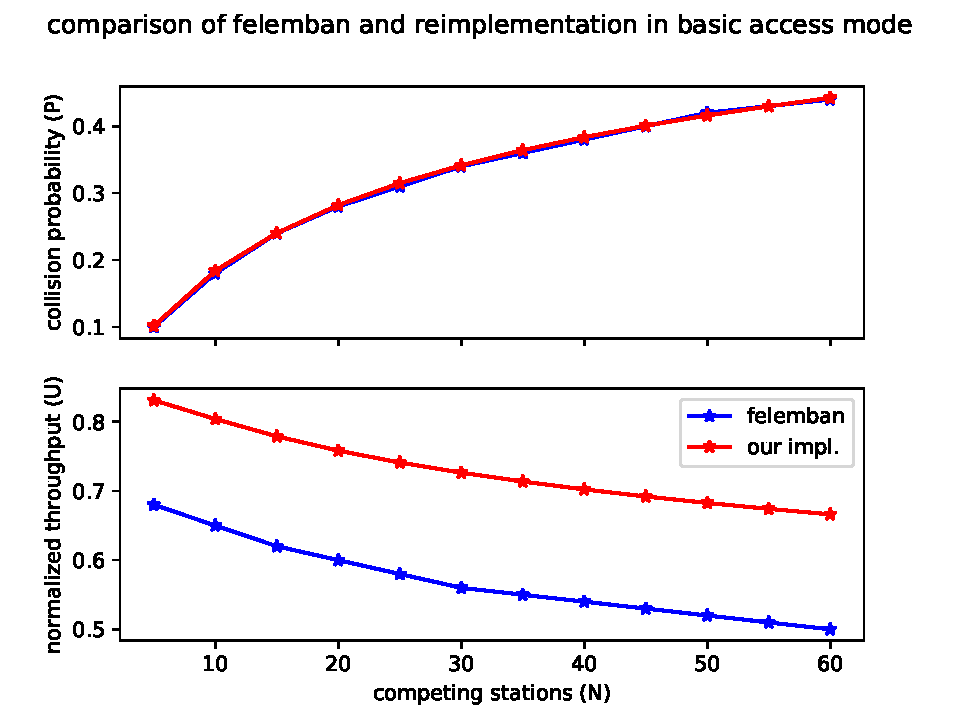
\includegraphics[width=0.8\textwidth]{images/reimpl.pdf}
  \caption{Our model reimplementation compared to values extracted from the original paper under similar network conditions.}
  \label{fig:modelimpl}
\end{figure}

To put this into perspective, at rougly 50 connected clients the conditional
packet collision probability reaches $40\%$, which results in a $0.4^{L+1}
\approx 0.06\%$ probability to fail transmission $L+1$ times and drop a
packet. At 20 clients, which is what we used during experiment 3, this falls
to $0.27^{L+1} \approx 0.003\%$.

Since clients are assumed to be identical, the packet drop probability for one
client and full network are equivalent. In Figure \ref{fig:relative_txfail_2g}
we show the total number of \texttt{tx\_fail}s (as reported to the kernel)
relative to the total number of packets transmitted, for 802.11 \emph{n}. Data
from 802.11 \emph{ac} is shown in Figure \ref{fig:relative_txfail_5g}. As seen
directly, the clients have a problem staying connected to the network throughout
the 802.11 \emph{n} test (indicated by lack of plots) and only few or no
packet drops were detected. The 802.11 \emph{ac} test, however, hovers around
the $0.003$, a full two orders of magnitude larger than the model's estimated
$0.003\%$.

\begin{figure}[tbp]
  \centering
  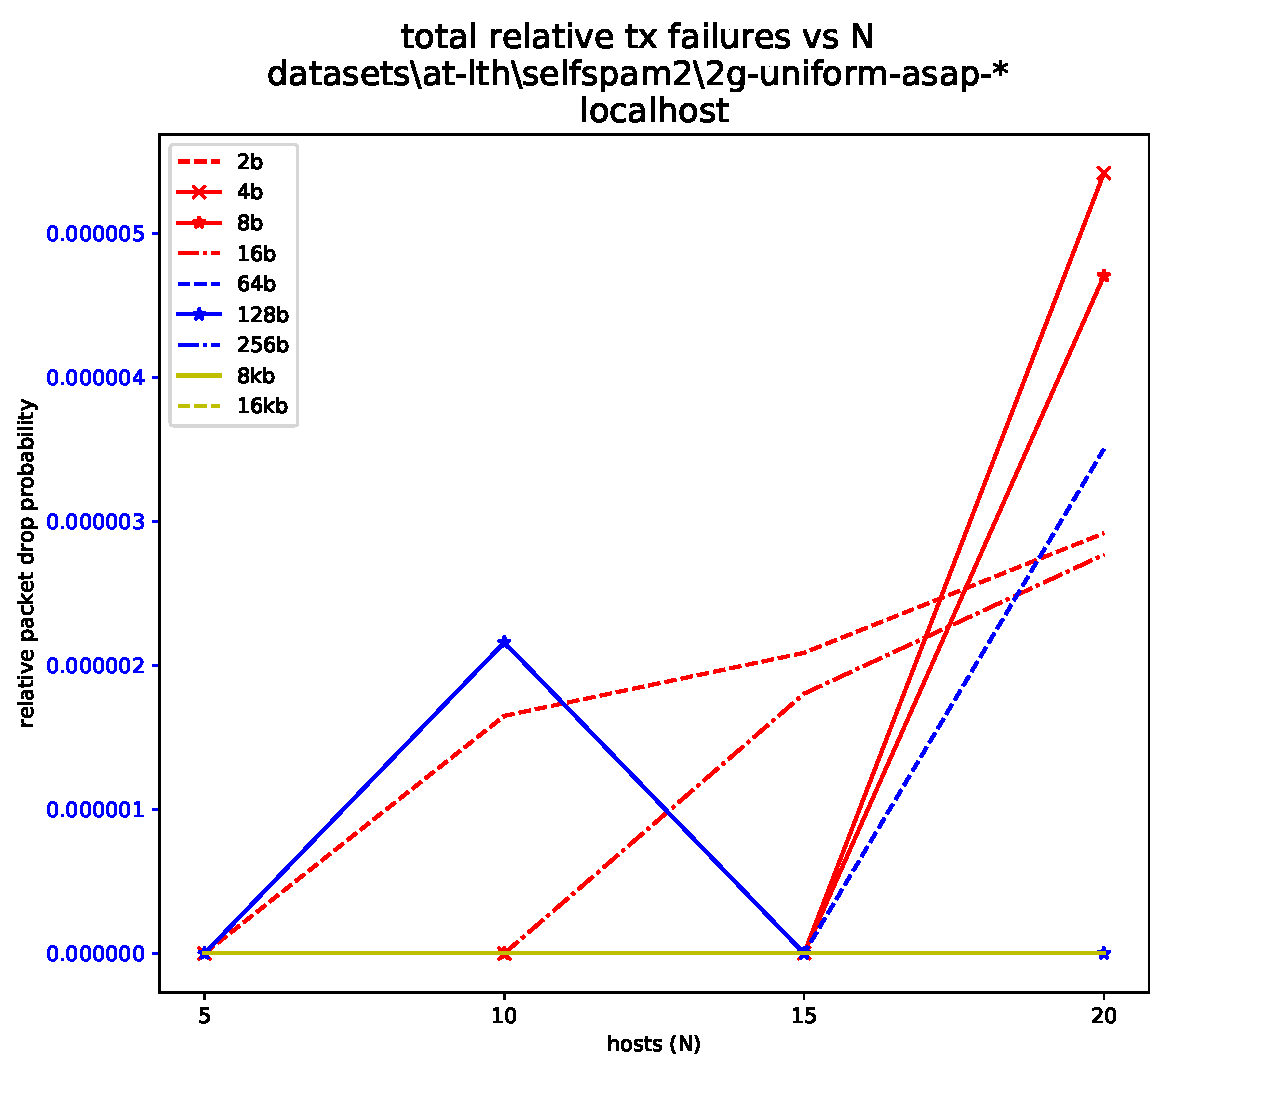
\includegraphics[width=0.8\textwidth]{images/relative_tx_fail_2g.pdf}
  \caption{Empirically obtained packet drop probability for 802.11 n.}
  \label{fig:relative_txfail_2g}
\end{figure}

\begin{figure}[tbp]
  \centering
  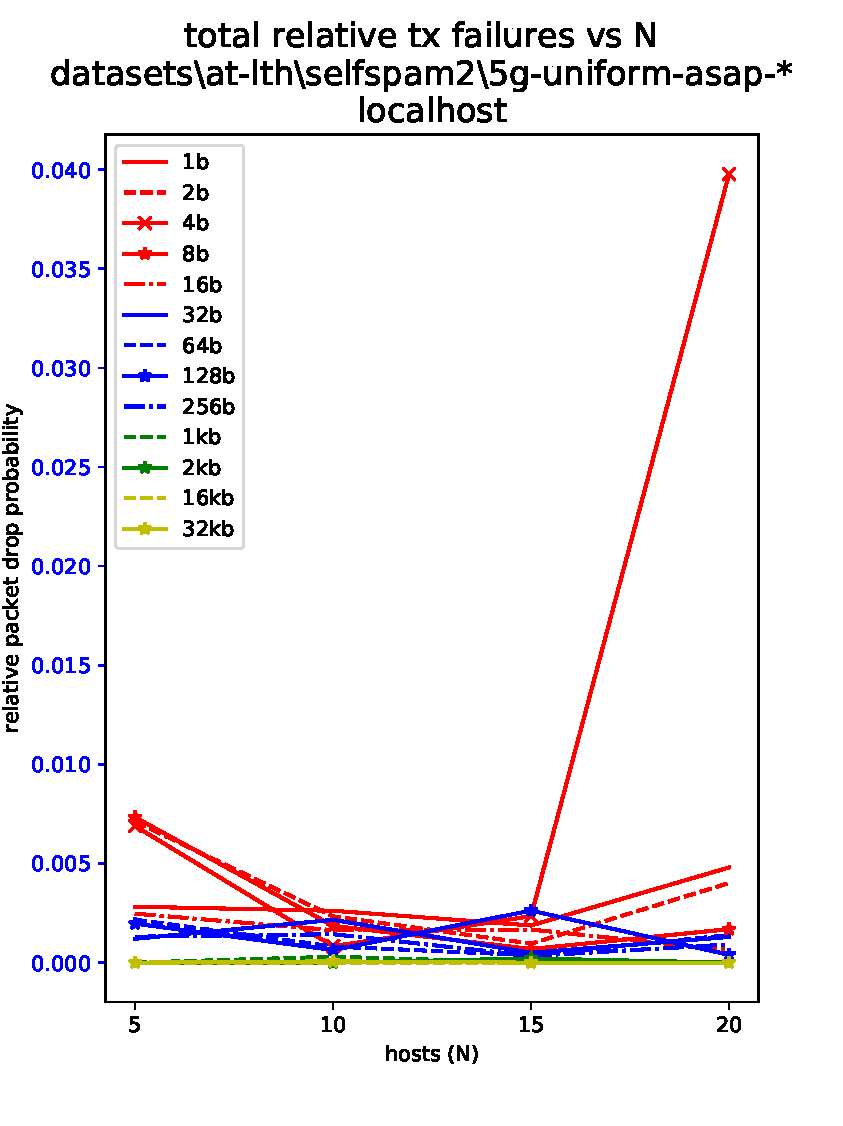
\includegraphics[width=0.8\textwidth]{images/relative_tx_fail_5g.pdf}
  \caption{Empirically obtained packet drop probability for 802.11 ac.}
  \label{fig:relative_txfail_5g}
\end{figure}

Finally, we tried to rescale and normalize the throughput by assuming that the
model was true. The model estimates about that at $N = 5$, normalized
throughput is at $68\%$, which puts channel capacity at
$\frac{\text{throughput}}{0.68}$. Figures \ref{fig:rescaled_tput_2g} and
\ref{fig:rescaled_tput_5g} show the (rescaled) normalized network throughput
(using the computed channel capacity), for varying $N$ and payload size. In
both figures, the cyan curve show the normalized throughput obtained from the
Felemban-Ekici paper with 1 KB payload at 1 Mbps (over 802.11 n).

\begin{figure}[tbp]
  \centering
  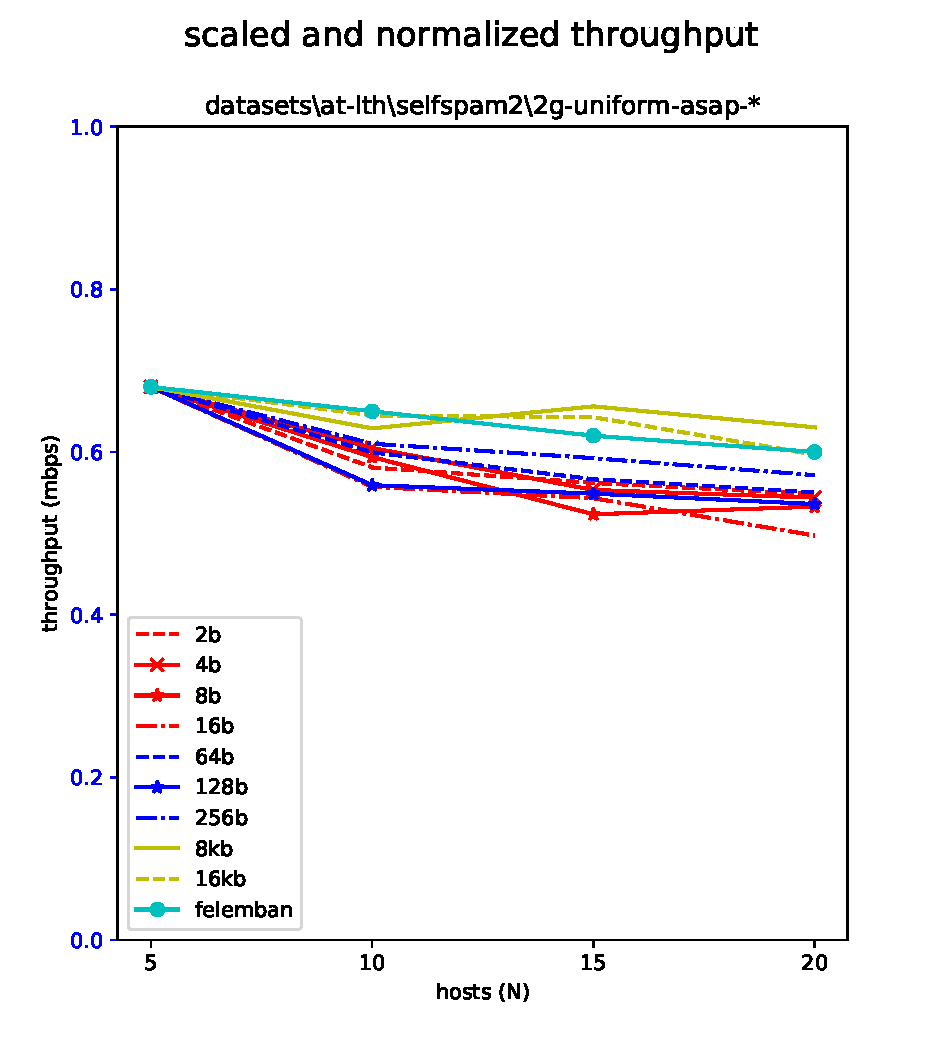
\includegraphics[width=0.8\textwidth]{images/rescaled_u_2g.pdf}
  \caption{Rescaled, (measured) normalized network throughput for 802.11 n compared with Felemban-Ekici.}
  \label{fig:rescaled_tput_2g}
\end{figure}

\begin{figure}[tbp]
  \centering
  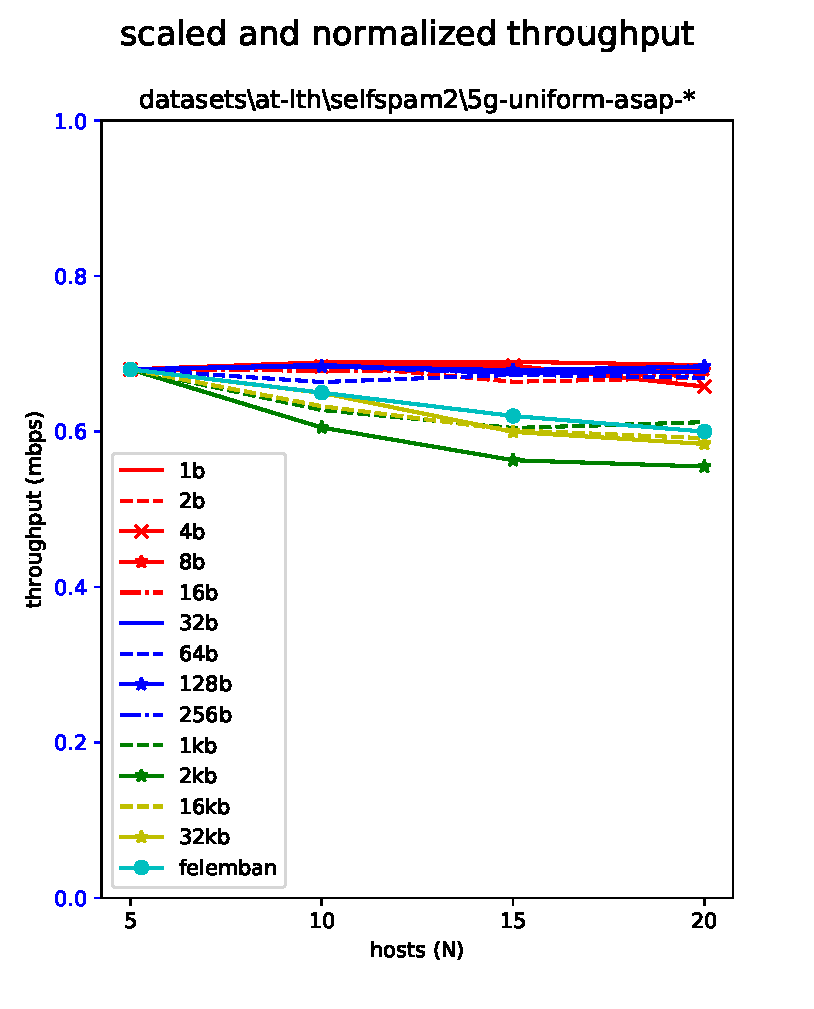
\includegraphics[width=0.8\textwidth]{images/rescaled_u.pdf}
  \caption{Rescaled, (measured) normalized network throughput during 802.11 ac compared with Felemban-Ekici.}
  \label{fig:rescaled_tput_5g}
\end{figure}

Figure \ref{fig:rescaled_tput_2g} (802.11 n) shows an expected behavior. Larger
payload sizes have higher relative utilization and roughly follow the
Felemban-Ekici curve. Lower payload sizes fall behind very fast. This hints at
a weakness in the model regarding different traffic flows.

Seemingly in opposition, Figure \ref{fig:rescaled_tput_2g} appears to imply
that smaller payload sizes incur no penalty as $N$ increases. Figure
\ref{fig:exp4throughput} reveals why, the throughput is already incredibly
low. Moving on, the larger payload sizes show similar curves compared to
802.11 n.

In conclusion, we cannot determine whether the predicted conditional packet
collision probability is correct or not. Although the model appears to predict
network throughput degredation as the number of connected nodes increase, it's
certainly not an apples to apples comparison. Our 802.11n network was mostly
stable at 72.2 (for raspberri pi 4's) and 200 Mbps on 802.11 ac, quite
different than model's 1 Mbps channel. As we could not generate normalized
throughput values from our reimplementation we cannot know what the output of
the model would have been for our network configurations.


\section{Future work}

\begin{itemize}

\item As seen in the network overview (Figure \ref{fig:linux_egress}) and
noticed during experiment 2, system call overhead and the userland/kernel
split have serious implications for latency-sensative measurements. An area
worth exploring is known as ``userland networking'' -- a technique common in
high-performance packet processing in which a userland application is allowed
exclusive access of a network device. Bypassing the kernel removes potential
bottlenecks such as context switches, memory allocation and copying,
scheduling and multithreading. In theory, this technique can reduce the number
of system calls of an application. More importantly, such an application can
design the communication between NIC and userland as a ring buffer,
eliminating the cost associated with memory allocation and deallocation
experienced in Experiment 2 (the unknown number of \texttt{to-be-freed}
packets).

\item An alternative approach to bypassing the kernel, is to bring the
userland program \emph{into} the kernel. The Berkley Packet Filter (BPF) is a
register-based filter evaluator designed for packet filtering
\cite{10.5555/1267303.1267305}. It has since been extended and redesigned
under the ``extended BPF'' (eBPF) moniker as an in-kernel virtual machine with
filters, taps and hooks all over the kernel. In short, the eBPF machine can
run arbitrary code inside the kernel, triggered by specific events. In theory,
this should allow for more accurate measurement of the packet transmission
process.


\item Continuing on the started path with a modified Wi-Fi driver, it would be
useful to also perform similar tests where the \texttt{jana} server also has
to reply back to the clients. These tests should more closely mimic the TCP
protocol upon which most of today's networking rely. Measuring the round trip
time (RTT) of packets and comparing the measured values with a modeled RTT (
based on IEEE 802.11 and TCP) could also lead to some interesting results.


\item And as is common practice today: when in doubt, throw machine learning
at the problem. While machine learning cannot enable more accurate
measurements, a machine-learning model could be trained to predict network
behaviour based on a large set of collected and labeled (as in, metric X
indicate outcome Y) metrics. A model may also be constructed for determining
possible user-friendly interventions (move device closer to router, the
channel is currently observing heavy interference so switch channel), however
an expert system (guided by real-time metrics) would probably be sufficient.
The system could be designed to run on each device (distributed) or on a
trusted machine (centralised). A centralised machine would have more
information to act on when issuing interventions back to users and,
potentially, directly to the Wi-Fi routers. Such a system could easily be
extended to record the outcome of any interventions (e.g. significantly
better or worse), possibly allowing for collection of data for unsupervised
machine learning.

During our thesis work we were able to identify several interesting metrics, available from \texttt{ubus}, such as number of connected clients, neighbouring
network data, medium availability, TX/RX PHY rates, RSSI, glitches and RTS settings. See \url{https://github.com/smeets/thesis/blob/master/paramlist.md} for more
parameters and their descriptions.


\end{itemize}

\section{Closing remarks \& thoughts}
This thesis primarily indicates that it currently is and most probably will become increasingly difficult to evaluate and use existing
models for practical Wi-Fi equipment. As the IEEE 802.11 specification evolves, newer Wi-Fi routers will always implement have new implementations and new features. At least, there are probably fewer chipset makers than router equipment
manufacturers.

Our attempts to obtain timing highly accurate packet timing data also show
that it requires a non-trivial amount of effort. It seems more likely that 
an overall measurement using ML/AI system is more easy to obtain for helping 
customers with the routers than trying to develop a system that works from the 
inside out as there are too many gaps between model and physical reality.  


		% \begin{thebibliography}{99}
		\bibliographystyle{plain}
		% \bibitem{bianchi} G. Bianchi, "Performance analysis of the IEEE 802.11 distributed coordination function" in {\it IEEE Journal on Selected Areas in Communications}, vol. 18, no. 3, pp. 535-547, March 2000.
		\bibliography{refs} 
		% \end{thebibliography}


	\appendix
% \chapter{Some extra material}
% \lipsum[1]

% \lstinputlisting[language=bash,caption={Router iperf3 script},label=lst:router]{../scripts/iperf_server.sh}

% \lstinputlisting[language=bash,caption={Client iperf3 script},label=lst:client]{../scripts/iperf_client.sh}

% \lstinputlisting[language=bash,caption={Router rssi logger script},label=lst:rssi]{../scripts/log_rssi.sh}

% \lstinputlisting[language=Python,caption={MDR parser},label=lst:mdrparse]{../scripts/mdrparser.py}

% \lstinputlisting[language=Python,caption={MDR heat map plotter},label=lst:mdrplot]{../scripts/mdr-plot.py}

% \lstinputlisting[language=Python,caption={Ekici-Felemban model implementation},label=lst:efmodel]{../models/felemban.py}

\end{document}
